\documentclass[12pt,addpoints,answers]{exam}
\usepackage[margin=1in]{geometry}
\usepackage{amsmath,amssymb,amsfonts}
\usepackage{graphicx}
\usepackage{float}
\usepackage[T1]{fontenc}
\usepackage[utf8]{inputenc}
\printanswers
\unframedsolutions

\begin{document}
\begin{center}
{\Large AP FRQ Pack}
\end{center}
\begin{questions}
\question
% q01-sgp02
Fish enter a lake at a rate modeled by the function $E$ given by $E(t) = 20 + 15 \sin\left(\frac{\pi t}{6}\right)$. Fish leave the lake at a rate modeled by the function $L$ given by $L(t) = 4 + 2^{0.1t^2}$. Both $E(t)$ and $L(t)$ are measured in fish per hour, and $t$ is measured in hours since midnight ($t = 0$).
\begin{parts}
\part How many fish enter the lake over the 5-hour period from midnight ($t = 0$) to 5 A.M. ($t = 5$)? Give your answer to the nearest whole number.
\part What is the average number of fish that leave the lake per hour over the 5-hour period from midnight ($t = 0$) to 5 A.M. ($t = 5$)?
\part At what time $t$, for $0 \le t \le 8$, is the greatest number of fish in the lake? Justify your answer.
\part Is the rate of change in the number of fish in the lake increasing or decreasing at 5 A.M. ($t = 5$)? Explain your reasoning.
\end{parts}
\begin{solution}
Part (a): $\int_0^5 E(t)\,dt = 153.457690$ \par To the nearest whole number, 153 fish enter the lake from midnight to 5 A.M. \par Part (b): $\frac{1}{5-0}\int_0^5 L(t)\,dt = 6.059038$ \par The average number of fish that leave the lake per hour from midnight to 5 A.M. is 6.059 fish per hour. \par Part (c): The rate of change in the number of fish in the lake at time $t$ is given by $E(t) - L(t)$. \par $E(t) - L(t) = 0 \Rightarrow t = 6.20356$ \par $E(t) - L(t) > 0$ for $0 \le t < 6.20356$, and $E(t) - L(t) < 0$ for $6.20356 < t \le 8$. Therefore the greatest number of fish in the lake is at time $t = 6.204$ (or 6.203). \par — OR — \par Let $A(t)$ be the change in the number of fish in the lake from midnight to $t$ hours after midnight. \par $A(t) = \int_0^t (E(s) - L(s))\,ds$ \par $A'(t) = E(t) - L(t) = 0 \Rightarrow t = C = 6.20356$ \par Therefore the greatest number of fish in the lake is at time $t = 6.204$ (or 6.203). \par Part (d): $E'(5) - L'(5) = -10.7228 < 0$ \par Because $E'(5) - L'(5) < 0$, the rate of change in the number of fish is decreasing at time $t = 5$.
\begin{center}
\begin{tabular}{|l|l|}
\hline
$t$ & $A(t)$ \\
\hline
0 & 0 \\
\hline
$C$ & 135.01492 \\
\hline
8 & 80.91998 \\
\hline
\end{tabular}
\end{center}
\par\medskip
\textbf{Scoring Guide}\par
Part (a): 2 : \{ 1 : integral, 1 : answer \} Part (b): 2 : \{ 1 : integral, 1 : answer \} Part (c): 3 : \{ 1 : sets $E(t) - L(t) = 0$, 1 : answer, 1 : justification \} Part (d): 2 : \{ 1 : considers $E'(5)$ and $L'(5)$, 1 : answer with explanation \}
\end{solution}

\question
% q02-sgp03
Let $S$ be the region bounded by the graph of the polar curve $r(\theta) = 3\sqrt{\theta}\sin\left(\theta^2\right)$ for $0 \le \theta \le \sqrt{\pi}$, as shown in the figure above.
\begin{center}
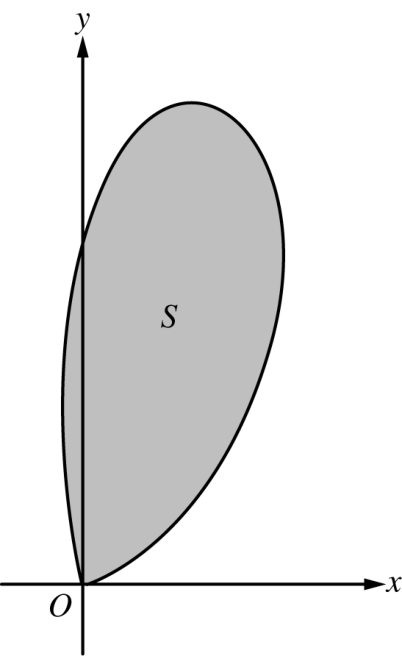
\includegraphics[width=0.8\linewidth]{figures/BC-2019_q2_fig_1.png}
\end{center}
\begin{parts}
\part Find the area of $S$.
\part What is the average distance from the origin to a point on the polar curve $r(\theta) = 3\sqrt{\theta}\sin\left(\theta^2\right)$ for $0 \le \theta \le \sqrt{\pi}$?
\part There is a line through the origin with positive slope $m$ that divides the region $S$ into two regions with equal areas. Write, but do not solve, an equation involving one or more integrals whose solution gives the value of $m$.
\part For $k > 0$, let $A(k)$ be the area of the portion of region $S$ that is also inside the circle $r = k\cos\theta$. Find $\lim_{k \to \infty} A(k)$.
\end{parts}
\begin{solution}
Part (a): $\frac{1}{2}\int_0^{\sqrt{\pi}} (r(\theta))^2 \, d\theta = 3.534292$ \par The area of $S$ is 3.534. \par Part (b): $\frac{1}{\sqrt{\pi} - 0}\int_0^{\sqrt{\pi}} r(\theta) \, d\theta = 1.579933$ \par The average distance from the origin to a point on the curve $r = r(\theta)$ for $0 \le \theta \le \sqrt{\pi}$ is 1.580 (or 1.579). \par Part (c): $\tan\theta = \frac{y}{x} = m \Rightarrow \theta = \tan^{-1}m$ \par $\frac{1}{2}\int_0^{\tan^{-1}m} (r(\theta))^2 \, d\theta = \frac{1}{2}\left(\frac{1}{2}\int_0^{\sqrt{\pi}} (r(\theta))^2 \, d\theta\right)$ \par Part (d): As $k \to \infty$, the circle $r = k\cos\theta$ grows to enclose all points to the right of the $y$-axis. \par $\lim_{k\to\infty} A(k) = \frac{1}{2}\int_0^{\pi/2} (r(\theta))^2 \, d\theta = \frac{1}{2}\int_0^{\pi/2} \left(3\sqrt{\theta}\sin(\theta^2)\right)^2 \, d\theta = 3.324$
\par\medskip
\textbf{Scoring Guide}\par
Part (a): 2 points: \{1 point: integral; 1 point: answer\} Part (b): 2 points: \{1 point: integral; 1 point: answer\} Part (c): 3 points: \{1 point: equates polar areas; 1 point: inverse trigonometric function applied to $m$ as limit of integration; 1 point: equation\} Part (d): 2 points: \{1 point: limits of integration; 1 point: answer with integral\}
\end{solution}

\question
% q03-sgp04
The continuous function $f$ is defined on the closed interval $-6 \le x \le 5$. The figure above shows a portion of the graph of $f$, consisting of two line segments and a quarter of a circle centered at the point $(5, 3)$. It is known that the point $(3, 3 - \sqrt{5})$ is on the graph of $f$.
\begin{center}
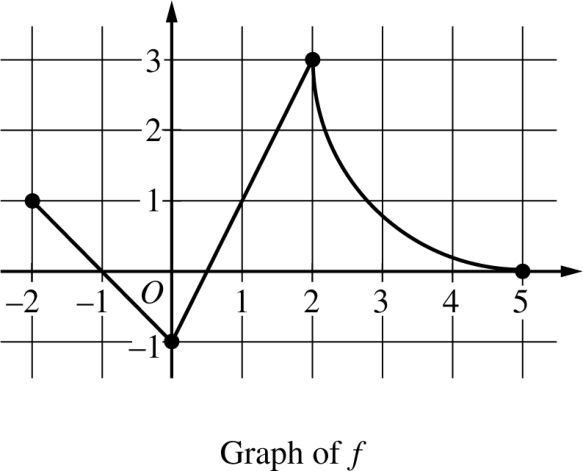
\includegraphics[width=0.8\linewidth]{figures/BC-2019_q3_fig_1.png}
\\ Graph of f
\end{center}
\begin{parts}
\part If $\int_{-6}^{5} f(x)\,dx = 7$, find the value of $\int_{-6}^{-2} f(x)\,dx$. Show the work that leads to your answer.
\part Evaluate $\int_{3}^{5} (2f'(x) + 4)\,dx$.
\part The function $g$ is given by $g(x) = \int_{-2}^{x} f(t)\,dt$. Find the absolute maximum value of $g$ on the interval $-2 \le x \le 5$. Justify your answer.
\part Find $\lim_{x \to 1} \frac{10^x - 3f'(x)}{f(x) - \arctan x}$.
\end{parts}
\begin{solution}
Part (a): $\int_{-6}^{5} f(x)\,dx = \int_{-6}^{-2} f(x)\,dx + \int_{-2}^{5} f(x)\,dx$ \par $\Rightarrow 7 = \int_{-6}^{-2} f(x)\,dx + 2 + \left(9 - \frac{9\pi}{4}\right)$ \par $\Rightarrow \int_{-6}^{-2} f(x)\,dx = 7 - \left(11 - \frac{9\pi}{4}\right) = \frac{9\pi}{4} - 4$ \par Part (b): $\int_{3}^{5} (2f'(x) + 4)\,dx = 2\int_{3}^{5} f'(x)\,dx + \int_{3}^{4} 4\,dx$ \par $= 2(f(5) - f(3)) + 4(5 - 3)$ \par $= 2(0 - (3 - \sqrt{5})) + 8$ \par $= 2(-3 + \sqrt{5}) + 8 = 2 + 2\sqrt{5}$ \par — OR — \par $\int_{3}^{5} (2f'(x) + 4)\,dx = [2f(x) + 4x]_{x=3}^{x=5}$ \par $= (2f(5) + 20) - (2f(3) + 12)$ \par $= (2 \cdot 0 + 20) - (2(3 - \sqrt{5}) + 12)$ \par $= 2 + 2\sqrt{5}$ \par Part (c): $g'(x) = f(x) = 0 \Rightarrow x = -1, x = \frac{1}{2}, x = 5$ \par Table of values: \par On the interval $-2 \le x \le 5$, the absolute maximum value of $g$ is $g(5) = 11 - \frac{9\pi}{4}$. \par Part (d): $\lim_{x \to 1} \frac{10^3 - 3f'(x)}{f(x) - \arctan x} = \frac{10^3 - 3f'(1)}{f(1) - \arctan 1}$ \par $= \frac{10 - 3 \cdot 2}{1 - \arctan 1} = \frac{4}{1 - \frac{\pi}{4}}$
\begin{center}
\begin{tabular}{|l|l|}
\hline
$x$ & $g(x)$ \\
\hline
$-2$ & $0$ \\
\hline
$-1$ & $\frac{1}{2}$ \\
\hline
$\frac{1}{2}$ & $-\frac{1}{4}$ \\
\hline
$5$ & $11 - \frac{9\pi}{4}$ \\
\hline
\end{tabular}
\end{center}
\par\medskip
\textbf{Scoring Guide}\par
Part (a): 3 points $1 : \int_{-6}^{5} f(x)\,dx = \int_{-6}^{-2} f(x)\,dx + \int_{-2}^{5} f(x)\,dx$ $1 : \int_{-2}^{5} f(x)\,dx$ $1 : $ answer Part (b): 2 points $1 : $ Fundamental Theorem of Calculus $1 : $ answer Part (c): 3 points $1 : g'(x) = f(x)$ $1 : $ identifies $x = -1$ as a candidate $1 : $ answer with justification Part (d): 1 point $1 : $ answer
\end{solution}

\question
% q04-sgp05
A cylindrical barrel with a diameter of 2 feet contains collected rainwater, as shown in the figure above. The water drains out through a valve (not shown) at the bottom of the barrel. The rate of change of the height $h$ of the water in the barrel with respect to time $t$ is modeled by $\frac{dh}{dt} = -\frac{1}{10}\sqrt{h}$, where $h$ is measured in feet and $t$ is measured in seconds. (The volume $V$ of a cylinder with radius $r$ and height $h$ is $V = \pi r^2 h$.)
\begin{center}
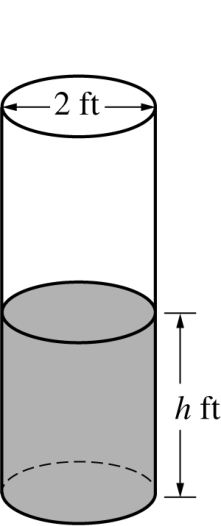
\includegraphics[width=0.8\linewidth]{figures/BC-2019_q4_fig_1.png}
\\ Cylindrical barrel with water
\end{center}
\begin{parts}
\part Find the rate of change of the volume of water in the barrel with respect to time when the height of the water is 4 feet. Indicate units of measure.
\part When the height of the water is 3 feet, is the rate of change of the height of the water with respect to time increasing or decreasing? Explain your reasoning.
\part At time $t = 0$ seconds, the height of the water is 5 feet. Use separation of variables to find an expression for $h$ in terms of $t$.
\end{parts}
\begin{solution}
Part (a): $V = \pi r^2 h = \pi(1)^2 h = \pi h$ \par $\frac{dV}{dt} = \pi\frac{dh}{dt}\bigg|_{h=4} = \pi\left(-\frac{1}{10}\sqrt{4}\right) = -\frac{\pi}{5}$ cubic feet per second \par Part (b): $\frac{d^2h}{dt^2} = -\frac{1}{20\sqrt{h}}\frac{dh}{dt} = -\frac{1}{20\sqrt{h}} \cdot \left(-\frac{1}{10}\sqrt{h}\right) = \frac{1}{200}$ \par Because $\frac{d^2h}{dt^2} = \frac{1}{200} > 0$ for $h > 0$, the rate of change of the height is increasing when the height of the water is 3 feet. \par Part (c): $\frac{dh}{\sqrt{h}} = -\frac{1}{10}dt$ \par $\int\frac{dh}{\sqrt{h}} = \int -\frac{1}{10}dt$ \par $2\sqrt{h} = -\frac{1}{10}t + C$ \par $2\sqrt{5} = -\frac{1}{10}(0) + C \Rightarrow C = 2\sqrt{5}$ \par $2\sqrt{h} = -\frac{1}{10}t + 2\sqrt{5}$ \par $h(t) = \left(-\frac{1}{20}t + \sqrt{5}\right)^2$
\par\medskip
\textbf{Scoring Guide}\par
Part (a): 2 points: 1 : $\frac{dV}{dt} = \pi\frac{dh}{dt}$ 1 : answer with units Part (b): 3 points: 1 : $\frac{d}{dh}\left(\frac{1}{10}\sqrt{h}\right) = -\frac{1}{20\sqrt{h}}$ 1 : $\frac{d^2h}{dt^2} = -\frac{1}{20\sqrt{h}}\cdot\frac{dh}{dt}$ 1 : answer with explanation Part (c): 4 points: 1 : separation of variables 1 : antiderivatives 1 : constant of integration and uses initial condition 1 : $h(t)$ Note: $0/4$ if no separation of variables Note: max $2/4$ [1-1-0-0] if no constant of integration
\end{solution}

\question
% q05-sgp06
Consider the family of functions $f(x) = \frac{1}{x^2 - 2x + k}$, where $k$ is a constant.
\begin{parts}
\part Find the value of $k$, for $k > 0$, such that the slope of the line tangent to the graph of $f$ at $x = 0$ equals 6.
\part For $k = -8$, find the value of $\int_0^1 f(x)\,dx$.
\part For $k = 1$, find the value of $\int_0^2 f(x)\,dx$ or show that it diverges.
\end{parts}
\begin{solution}
Part (a): $f'(0) = \frac{2}{k^2} = 6 \Rightarrow k^2 = \frac{1}{3} \Rightarrow k = \frac{1}{\sqrt{3}}$ \par Part (b): $\frac{1}{x^2 - 2x - 8} = \frac{1}{(x - 4)(x + 2)} = \frac{A}{x - 4} + \frac{B}{x + 2}$ \par $\Rightarrow 1 = A(x + 2) + B(x - 4)$ \par $\Rightarrow A = \frac{1}{6}, B = -\frac{1}{6}$ \par $\int_0^1 f(x)\,dx = \int_0^1 \left(\frac{1}{6(x - 4)} - \frac{1}{6(x + 2)}\right)\,dx$ \par $= \left[\frac{1}{6}\ln|x - 4| - \frac{1}{6}\ln|x + 2|\right]_{x=0}^{x=1}$ \par $= \left(\frac{1}{6}\ln 3 - \frac{1}{6}\ln 3\right) - \left(\frac{1}{6}\ln 4 - \frac{1}{6}\ln 2\right) = -\frac{1}{6}\ln 2$ \par Part (c): $\int_0^2 \frac{1}{x^2 - 2x + 1}\,dx = \int_0^2 \frac{1}{(x - 1)^2}\,dx = \int_0^1 \frac{1}{(x - 1)^2}\,dx + \int_1^2 \frac{1}{(x - 1)^2}\,dx$ \par $= \lim_{b \to 1^-} \int_0^b \frac{1}{(x - 1)^2}\,dx + \lim_{b \to 1^+} \int_b^2 \frac{1}{(x - 1)^2}\,dx$ \par $= \lim_{b \to 1^-} \left[-\frac{1}{x - 1}\right]_{x=0}^{x=b} + \lim_{b \to 1^+} \left[-\frac{1}{x - 1}\right]_{x=b}^{x=2}$ \par $= \lim_{b \to 1^-} \left(-\frac{1}{b - 1} - 1\right) + \lim_{b \to 1^+} \left(-1 + \frac{1}{b - 1}\right)$ \par Because $\lim_{b \to 1^-} \left(-\frac{1}{b - 1}\right)$ does not exist, the integral diverges.
\par\medskip
\textbf{Scoring Guide}\par
Part (a): 3 points \{ 1 : denominator of $f'(x)$ 1 : $f'(x)$ 1 : answer \} Part (b): 3 points \{ 1 : partial fraction decomposition 1 : antiderivatives 1 : answer \} Part (c): 3 points \{ 1 : improper integral 1 : antiderivative 1 : answer with reason \}
\end{solution}

\question
% q06-sgp07
A function $f$ has derivatives of all orders for all real numbers $x$. A portion of the graph of $f$ is shown above, along with the line tangent to the graph of $f$ at $x = 0$. Selected derivatives of $f$ at $x = 0$ are given in the table above.
\begin{center}
\begin{tabular}{|l|l|}
\hline
$n$ & $f^{(n)}(0)$ \\
\hline
2 & 3 \\
\hline
3 & $-\frac{23}{2}$ \\
\hline
4 & 54 \\
\hline
\end{tabular}
\end{center}
\begin{center}
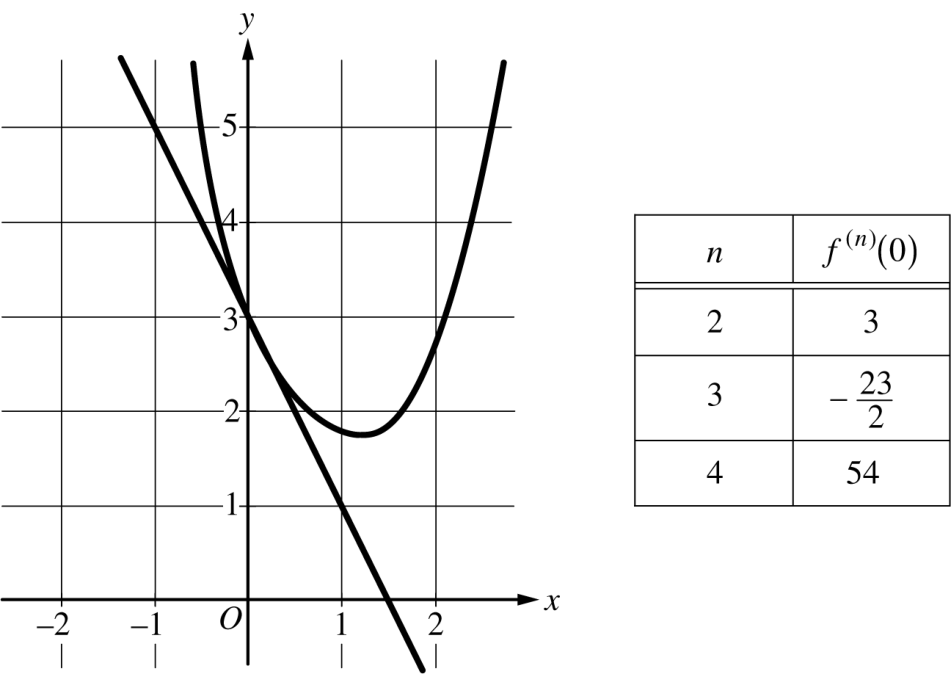
\includegraphics[width=0.8\linewidth]{figures/BC-2019_q6_fig_1.png}
\end{center}
\begin{center}
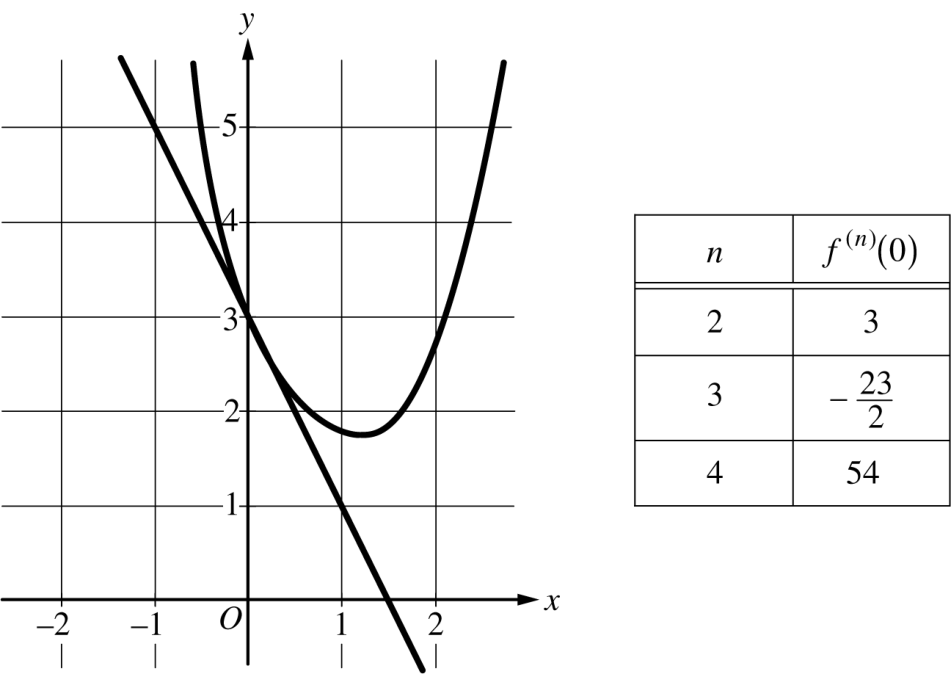
\includegraphics[width=0.8\linewidth]{figures/BC-2019_q6_fig_2.png}
\end{center}
\begin{parts}
\part Write the third-degree Taylor polynomial for $f$ about $x = 0$.
\part Write the first three nonzero terms of the Maclaurin series for $e^x$. Write the second-degree Taylor polynomial for $e^x f(x)$ about $x = 0$.
\part Let $h$ be the function defined by $h(x) = \int_0^x f(t) \, dt$. Use the Taylor polynomial found in part (a) to find an approximation for $h(1)$.
\part It is known that the Maclaurin series for $h$ converges to $h(x)$ for all real numbers $x$. It is also known that the individual terms of the series for $h(1)$ alternate in sign and decrease in absolute value to $0$. Use the alternating series error bound to show that the approximation found in part (c) differs from $h(1)$ by at most $0.45$.
\end{parts}
\begin{solution}
Part (a): $f(0) = 3$ and $f'(0) = -2$. The third-degree Taylor polynomial for $f$ about $x = 0$ is $3 - 2x + \frac{3}{2!}x^2 + \frac{-23}{3!}x^3 = 3 - 2x + \frac{3}{2}x^2 - \frac{23}{12}x^3$. \par Part (b): The first three nonzero terms of the Maclaurin series for $e^x$ are $1 + x + \frac{1}{2!}x^2$. The second-degree Taylor polynomial for $e^x f(x)$ about $x = 0$ is $3\left(1 + x + \frac{1}{2!}x^2\right) - 2x(1 + x) + \frac{3}{2}x^2(1) = 3 + (3-2)x + \left(\frac{3}{2} - 2 + \frac{3}{2}\right)x^2 = 3 + x + x^2$. \par Part (c): $h(1) = \int_0^1 f(t)\,dt \approx \int_0^1\left(3 - 2t + \frac{3}{2}t^2 - \frac{23}{12}t^3\right)dt = \left[3t - t^2 + \frac{1}{2}t^3 - \frac{23}{48}t^4\right]_{t=0}^{t=1} = 3 - 1 + \frac{1}{2} - \frac{23}{48} = \frac{97}{48}$. \par Part (d): The alternating series error bound is the absolute value of the first omitted term of the series for $h(1)$. $\int_0^1\left(\frac{54}{4!}t^4\right)dt = \left[\frac{9}{20}t^5\right]_{t=0}^{t=1} = \frac{9}{20}$. Error $\le \left|\frac{9}{20}\right| = 0.45$.
\par\medskip
\textbf{Scoring Guide}\par
Part (a): 2 points: \{1 point: two terms; 1 point: remaining terms\} Part (b): 2 points: \{1 point: three terms for $e^x$; 1 point: three terms for $e^x f(x)$\} Part (c): 2 points: \{1 point: antiderivative; 1 point: answer\} Part (d): 3 points: \{1 point: uses fourth-degree term of Maclaurin series for $f$; 1 point: uses first omitted term of series for $h(1)$; 1 point: error bound\}
\end{solution}
\end{questions}
\end{document}
